% Chapter 3

\chapter{WiSARDNet Cyberinfrastructure} % Write in your own chapter title
\label{Chapter 3}
\lhead{} % Write in your own chapter title to set the page header

\section{Overview}
This chapter describes the platform on which the work of this thesis is built. WiSARDNet is a WSN platform which consists of hardware and software that connect sensor/actuator nodes to users and their ecological experiments. Cyberinfrastructure describes computational systems with advanced data acquisition, processing, and management capabilities, according to one of the more widely used definitions of the term ~\cite{stewart10}. According to this definition, WiSARDNet can be thought of as cyberinfrastructure. Each network component is described in this chapter, as well as the data management and archival processes. The cyberinfrastructure hardware and software components can be divided into four categories: WSN, base station, real-time data center (RTDC), and end-user. Figure \ref{fig:device_hierarchy} shows how the hardware and software components for each of these categories fit together. The core component which links the WSN, the base station, and the real-time data center is a TCP/IP based message broker that uses the MQTT protocol. MQTT will be described in further detail in this chapter. Additionally, database archival components will be described in terms of their role in the cyberinfrastructure in this chapter. The technical specifics of the database will be described in greater detail in Chapter 4.\\

\begin{figure}[H]
	\centering
	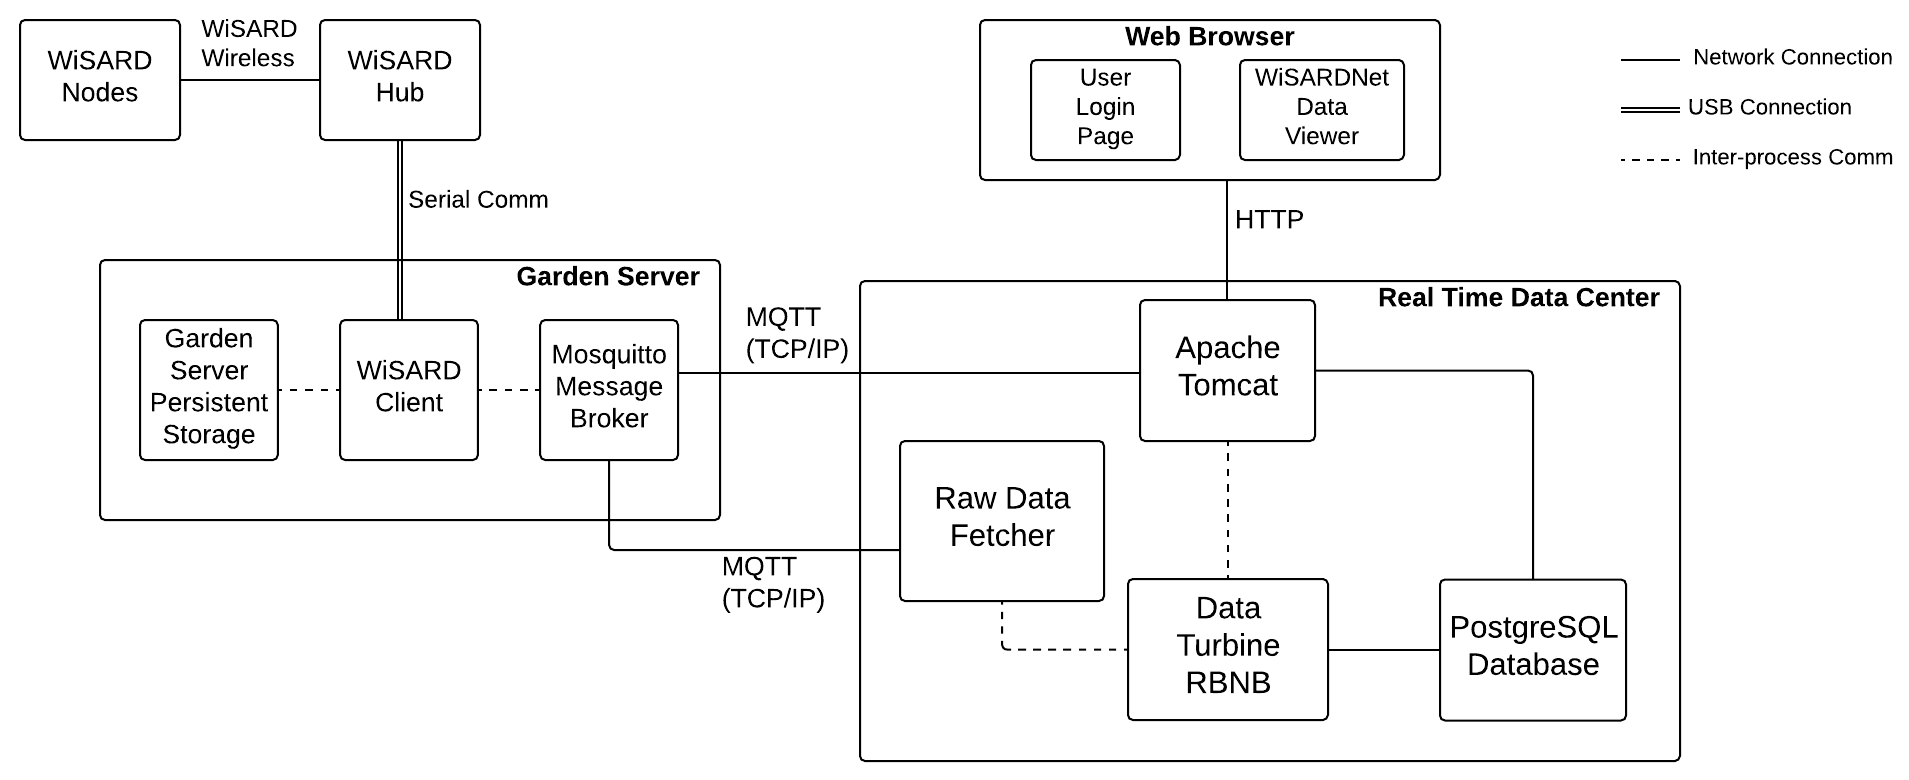
\includegraphics[width=\textwidth]{figures/wisardnet_ci_final}
	\caption{Cyberinfrastructure hardware and software component hierarchy}
	\label{fig:device_hierarchy}
\end{figure}

\section{WiSARD Nodes}
A Wireless Sensor/Actuator and Relay Device (WiSARD) is  modular, adapting easily to the different sensing and actuation needs of users. Flexibility and energy awareness are the two driving design motivations in the WiSARD development. At the heart of each WiSARD device is a central processor (CP) which governs the operation of the device and its peripherals. The CP dictates when and how tasks will be scheduled and executed, establishes and manages wireless links to other WiSARDs, facilitates the storage of sensor readings, and offloads the sensing and actuation tasks to daughterboards called satellite processors (SP).

A WiSARD can accommodate up to four different SPs. This enables each WiSARD to perform a variety of tasks specifically tailored to meet the needs of researchers and experimenters. There are three different types of SPs that a WiSARD can use: SP-ST, SP-STM, and SP-CM-STM. The SP-ST (SP - Sense Temperature) generates temperature readings by sampling Type-T thermocouples. The SP-STM (SP - Sense Temperature and Moisture) generates soil moisture and soil temperature samples. The SP-CM-STM (SP - Control Moisture - Sense Temperature and Moisture) accommodates the same sensing capabilities as the SP-STM but also provides water valve actuation capabilities. The modular design of the WiSARD allows the CP to offload these sensing and actuation operations to its SPs which can execute tasks in parallel with CP operation.

Both CP and SPs use a Texas Instruments MSP430 16-bit ultra-low-power microcontroller. This microcontroller has a variety of features and can be placed in various low-power modes. The low-power modes of operation, accompanied by energy-conscious software design, allow for a WiSARD to operate on a single pack of three AAA batteries for many weeks or even months, depending on the rate at which the devices dispatch their sampling operations. The CP also connects to a radio board which uses an Analog Devices ADF7020 RF transceiver module that operates in the 902-928 MHz license-free ISM band.  When WiSARDs are powered up, they autonomously form a self-organizing and self-healing multi-hop wireless ad-hoc network~\cite{Flikkema}. A special WiSARD which is assigned the software role of Hub acts as the base station, and is connected to an embedded Linux computer referred to as a garden server. 

\section{Middleware}

%The central architectural component which connects the garden servers to the RTDC is an open-source data streaming middleware software named Data Turbine. Data Turbine can be thought of as a data streaming engine acting as a ring-bufferred network bus (RBNB) which is a versatile and portable data streaming solution. Middleware software solutions operate under one of two operational paradigms: request/response or publish/subscribe. RBNB is a data broker which operates under the request/response paradigm of middleware software.  From an architectural standpoint, there are 3 core components to a Data Turbine implementation: servers, sources, and sinks. The Data Turbine server houses the actual data structure which manages the data and makes it available for request. Data Turbine Source objects aggregate data for insertion into the Data Turbine server. Alternatively, Data Turbine sink objects request data from the Data Turbine server and make it available to the process or user that desires it. Data turbine was written in Java, and is therefore versatile in the number of platforms upon which servers, sources, and sinks can execute. This, as well as the Data Turbine application programming interface (API) allows for a variety of data-centric applications and experiments to be performed. 

Middleware is a term which describes a software abstraction of the transfer of information from point A to  point B. By hiding the complexities of data transport behind a simple interface that connects two pieces of software, the development of powerful data processing and management tools can be accelerated. WiSARDNet relies heavily upon the use of middleware to make the WSN data available to the rest of the world. The central architectural component that connects the garden servers to the RTDC is MQTT. MQTT is a data transfer protocol created by IBM that utilizes the publish/subscribe middleware paradigm~\cite{HunTruSta08}.

In order for MQTT to be explained in the context of this work, a few more terms need to be defined. This work is concerned with the reconfiguration of WiSARD nodes. Each WiSARD is comprised of multiple devices. A device is a singular piece of hardware; a transducer, a CP, a SP, and a radio are each examples  of a device. The set of operational parameters that control a device is called a configuration. A deployment is an instance of a device and its configuration. Reconfiguration is the process of changing the operational parameters of one or more deployed devices.

MQTT facilitates the sharing of data between applications through the use of brokers. A broker is an application that sends and receives data to and from other applications. The transferred data are called messages. When a program sends a message to a broker, it labels the message with a topic name. The program sending the message is called a publishing client. A program that is interested in data from a publishing client can subscribe to a topic through the broker; this program is called a subscription client. All messages from publishing clients that are labeled with a matching topic will be sent by the broker to all subscription clients that have subscribed to that topic.

WiSARDNet uses Mosquitto~\cite{mosquitto}, an open source implementation of a message broker that uses the MQTT protocol. A message broker installed on each garden server keeps all of the data from that site in non-volatile memory. The data is organized into archive files at regular time intervals. To transfer the data from the WiSARDs to the broker, a Java application referred to as a WiSARD client uses MQTT messages to publish data. The RTDC can then retrieve the data using a subscription client that connects to the garden server message brokers over cellular or satellite connections.

An MQTT subscription client for each garden site runs at the RTDC and is responsible for subscribing to all the data published to each broker. These subscription clients are what is referred to in WiSARDNet as a raw data fetcher (RDF).  The purpose of the RDFs is to retrieve all of the data from all of the gardens so that the data is accessible for processing, storage, or viewing. These processes are discussed in detail in the following section.

%Within the WiSARDNet CI, each garden server runs a local instance of the Data Turbine server. Data Turbine Source objects are small software programs which funnel data gathered from the local WiSARD network feed data into the Data Turbine server. Alternatively, sink objects pull data out of the Data Turbine server. Data Turbine uses what is referred to as a channel map as a means to associate individual data channels with the Data Turbine streams that connect sources and sinks to the Data Turbine server. At the RTDC, a much larger instance of the Data Turbine server runs, with source objects connecting to each garden server. By initializing a Data Turbine sink, a user or application may request specifically identified data channels from the Data Turbine server using a channel map with the names defined by the user in the source. In the WiSARDNet CI, the Data Turbine server at the RTDC requests all new data at regular intervals from the Data Turbine server instances at each garden, and inserts the data into a single central location. These requests are made via TCP/IP connections between the garden servers and the RTDC via their cellular or satellite based Internet connections. The WiSARDs themselves are not directly ip-addressable and therefore funneling data to the RTDC via each garden's base station greatly simplifies the procedure of requesting data from each location.

\section{Real-time Data Center}
The RTDC is a collection of compute and data servers that host a Apache Tomcat web server, a Mosquitto MQTT subscription client, an instance of an open-source data streaming middleware called Data Turbine, a PostgreSQL relational database, and all of the data management processes and applications which interact with the WSN. The RTDC has several functions, the first of which is to retrieve all of the WSN data from each of the gardens. The RTDC is a centralized destination for all of the network's data streams. From this location, applications can access, store, and modify data for their various needs, as opposed to having to interact with multiple networks individually. For instance, a process which reads in raw data streams from temperature sensors might need to calculate human-readable values from the raw sensor readings. A single data converting processor which moves data from raw transducer values to human-readable values, can easily acquire all of the raw data streams for temperature sensors at all network locations with a single fetch, rather than requiring that the process fetch the raw data from each specific garden individually. Additionally, aggregating all data at the RTDC greatly simplifies archival and backup procedures.

Another function that the RTDC performs is the execution of applications and processes which interact with the WSNs and their data. One example of an application running on a server at the RTDC might be an experiment which attempts to maintain equal soil moisture readings at two different geographic locations. The RTDC servers possess high-performance computing hardware that many applications and processes can use to interact  with the networks in real-time.

\subsection{Relational Database}
Relational databases provide a flexible way to store and access large amounts of data. A relational database is composed of one or more tables; tables are 2 dimensional matrices of rows and columns. According to Rockoff ~\cite{rockoff2010language}, rows and columns are referred to as records and fields, respectively. An entry in a database table occupies a single row and each field corresponding to a different attribute of that entry constitutes a new column. For example, a table which stores people might have columns for an identification number, a name, an address, and a telephone number. An entry of a new person into this table would occupy a single row, with the data matching each of the attributes would occupy the rows' intersections with each column. Formally, these columns are referred to as primary keys, as they uniquely identify database records. The database at the RTDC has numerous tables which store information about every device, garden location, and sensor reading.

In WiSARDNet, data streams are archived in a PostgreSQL table. Other tables in this database store all of the meta-data and logistical information regarding all WSN devices, as well as every data point sampled from all transducers. Additionally, there are many data streams that need to be tracked and archived such as diagnostic and control data, error reporting, and other useful information. An example of diagnostic data might be the logging of a device restart event; such events can be crucial in detecting and analyzing network performance issues.

The PostgreSQL database where all of this data is archived is physically located on its own server hardware at the RTDC, separate from the other data management and processing clients. By placing the database on its own server hardware, the database has exclusive access to dedicated processing resources to allow for the quickest possible query and insert times. 

\subsection{Data Schema}
WiSARD devices interact according to the relationships that result from how they are connected together. Figure \ref{fig:device_hierarchy_edit} shows a set of device relationships for an example WiSARD. The example WiSARD uses three different SP types, each one accommodating specific transducers or actuators. 

\begin{figure}[H]
	\centering
	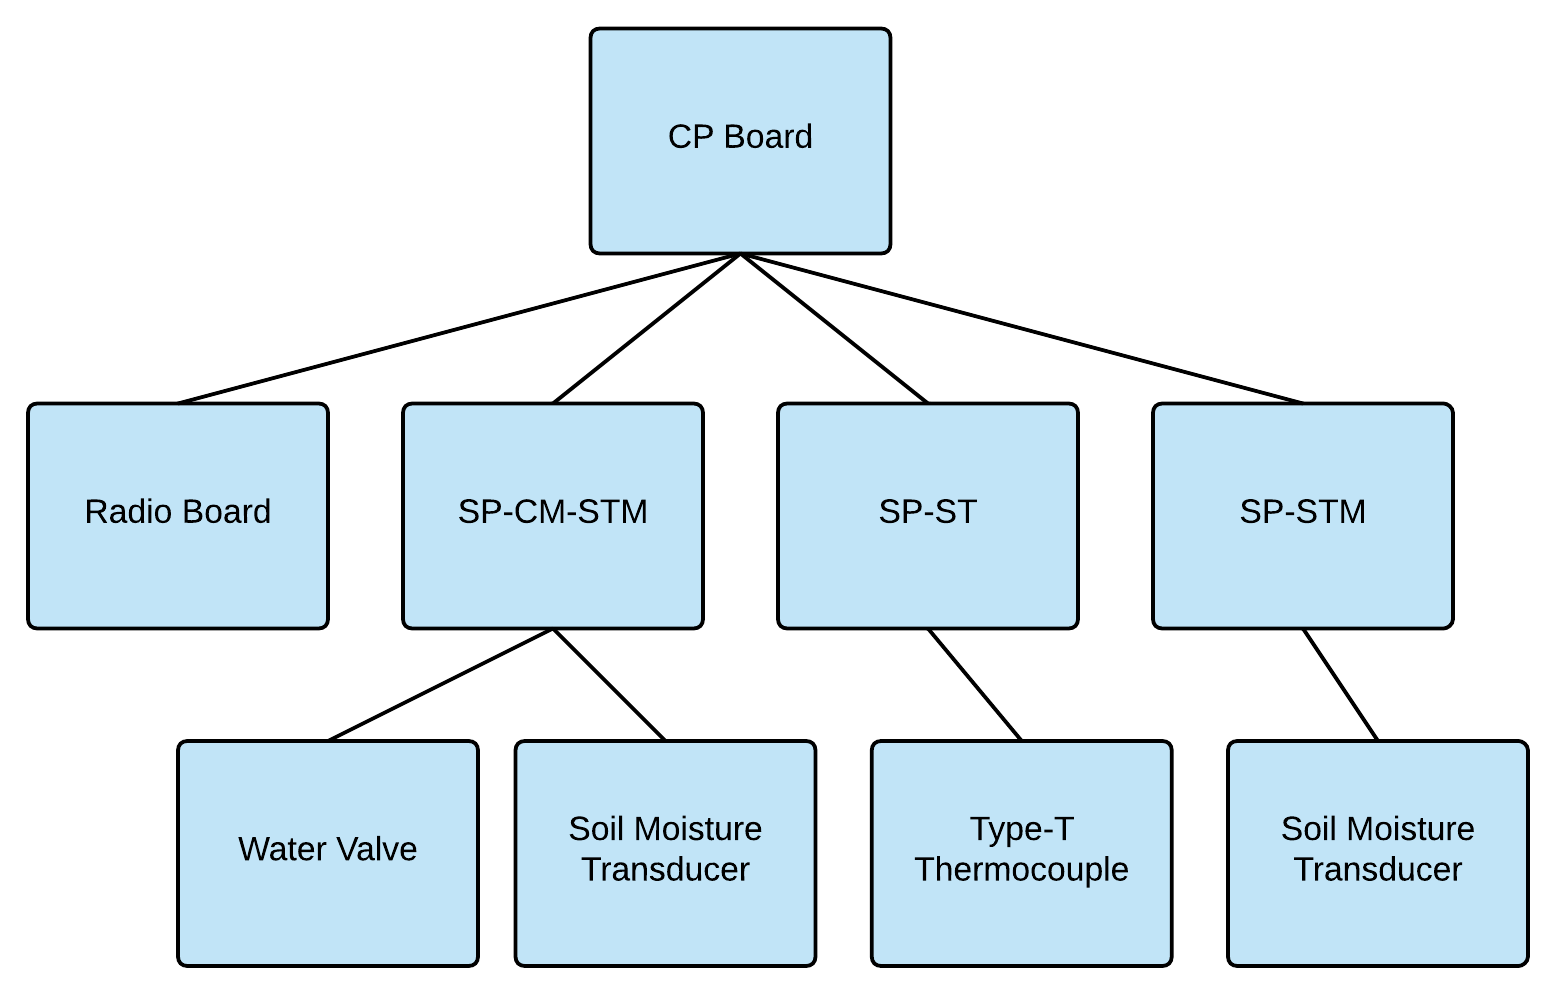
\includegraphics[width=\textwidth]{figures/wisard_device_hierarchy.png}
	\caption{Example of a WiSARD's device relationship structure. This WiSARD has three SPs and each SP has a transducer. The SP-CM-STM also has a water valve that it actuates.}
	\label{fig:device_hierarchy_edit}
\end{figure}

WiSARDNet organizes gathered data into database tables in a way that accommodates the reconfiguration of WiSARDNet devices. The organizational structures and relationships of the database tables are known as the database schema. Every piece of hardware is referred to in the schema as a device. The Device Table is therefore an important table in the schema. A record in the Device Table describes any device of any type. For instance, a radio, a soil-moisture transducer, a satellite processor, or a garden server are all types of devices that each have records in the Device Table. The configuration of a device might change at some point in time; it might be moved to another location, it might be upgraded or replaced, or it might receive a new firmware version. In this schema, the device's software parameters, hardware configuration, and state of operation are all encapsulated in a deployment. All deployments are stored as records in the Deployment Table.

When a transducer is attached to a SP, then its deployment record references the SP's deployment record in the Parent deployment field. When a change is made to any of the parameters tracked in the deployment table, the device is considered to have a new deployment, and therefore a new record is inserted into the deployment table. Both the old and new deployment records reference the device record, but the old deployment is disabled by setting the Active deployment field to \textit{false}. Over time, many deployment records may accumulate for a particular device as changes are made. However, there should only ever be one active deployment for a device at any given time. This allows the entire deployment history of a device to be stored so that all data points from a device can be correlated to the configuration of the device at the time that the data point was created. Currently the rule of having only one active deployment for a device at any given time is not enforced by the database. Instead, this is governed by the procedures followed by a technician or researcher when creating a new deployment.

A WiSARD's device relationships naturally form a tree structure. The reason for this is because a WiSARD has exactly one CP to which all other devices connect, either directly or indirectly. This resembles the concept of a root node in a tree data structure. Likewise, each SP resembles the internal nodes of a tree since it connects to at most one CP, but can be parent to multiple transducers or actuators. Finally, the radio, the transducers, and the actuators resemble the leaf nodes of a tree since they cannot be parent to any other devices. The database schema reflects the tree structure by storing the device deployment records with parent/child relationships. This allows all of the devices of a WiSARD to be accessed using standard tree traversal algorithms on the device Deployment Table records.

%Figure \ref{fig:deployment_hierarchy_edit} shows how devices and deployments are structured in the database. Each deployment record has a field for a parent device deployment. 

%\begin{figure}[H]
%	\centering
%	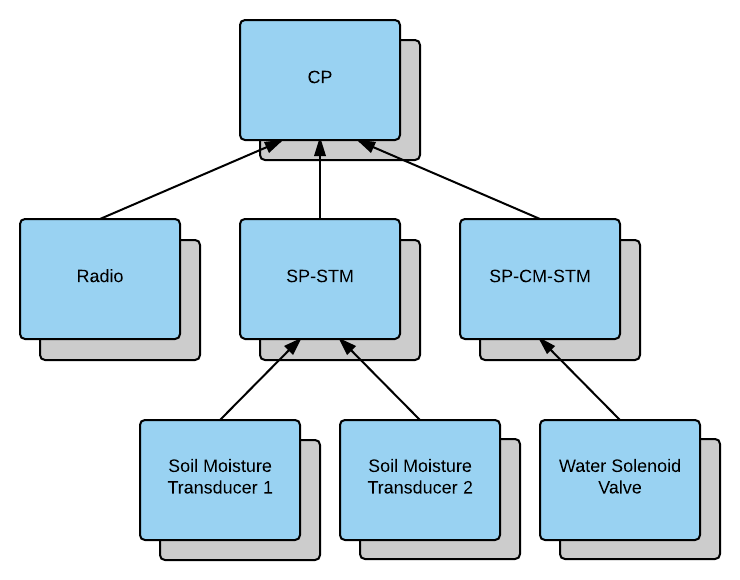
\includegraphics[width=\textwidth]{figures/deployment_hierarchy.png}
%	\caption{A visual showing each device (background) and its active deployment (foreground) and how the deployments are connected}
%	\label{fig:deployment_hierarchy_edit}
%\end{figure}

Having the ability to store and track each device's configuration and related metadata in the database is of great value in the management of the networks and the various experiments. When a WiSARD is ready for deployment at a garden site, a deployment record is created with all of its configuration data, the deployment record is set to active, and the start date and time is set. As long as the device remains in this configuration, the deployment object pointing to that device will remain active. If a device is changed in any substantive way, the following actions are taken:

\begin{enumerate}
	\item The deployment record referencing the changed device is set to inactive.
	\item The current time is inserted into the stop-time field of the deployment record
	\item A new deployment record is inserted into the deployment table
	\item The parent field of the new deployment record references the deployment record of the parent device
	\item The active status field of the new deployment record is set to active
	\item The current time is inserted into the start-time field of the new deployment record
\end{enumerate}

By following this procedure, device configurations are easily accessible from the database. A previous deployment exists as a single record in the Deployment Table which is trivial with regards to computational complexity and storage resources. This approach is simple, intuitive, and scales well as the number of devices deployed in the field increase. With this paradigm, a data sample is not merely a sample from a device,  it is a sample from a specific deployment of a device. When a device's configuration is altered, a new deployment is created for that device and the data generated by that device references the new deployment record.

When new data from WiSARDs arrive at the RTDC from the MQTT broker, they need to be accessible for users and other services to request. Data Turbine's network accessible ring buffer data structure works well for this purpose. At the RTDC, the data streams arriving via MQTT are placed into Data Turbine's ring buffer in accordance with the stream name which identifies the device from which the sample was taken. Since the complexities of WiSARD configurations are handled via storing their configuration data in database tables, archival of sampled data in the database becomes a simple procedure. All samples from all streams are placed as individual records in a table named Data. In addition to the sampled value and the time that it was sampled, the value can be related to the specific device and deployment records via its Data Turbine stream name. In this way, data archival of acquired samples is extremely simple and all information regarding a device and its samples is easily accessible and intuitively obtained through the thoughtful design of the data schema. 

\section{Summary}
WiSARDNet is a WSN CI which was designed from the ground up to be modular, scalable, and accessible to users. The Mosquitto MQTT broker, the data streaming middleware Data Turbine, and the RTDC enable data sampled by sensors to be retrieved, managed, processed, and archived into a PostgreSQL database. The way in which WiSARD meta-data and configuration information is stored and accessed is critical for the development of a network configuration software which comprises the work of this thesis. How these features are utilized in the network management software is described in further detail in Chapter 4.